\section{QAES}

\begin{frame}{QAES\footfullcite{aeslowmc}}
\begin{itemize}
    \item Authors compared various previously proposed Sbox designs on the G-cost and DW-cost metrics by reconstructing them.
    \pause
    \item \cite{aessbox} Sbox was effective in terms of G-cost and DW-cost hence they chose it.
    \begin{center}
    \pause
\begin{table}[h!]
    \centering
    \resizebox{8cm}{!}{\begin{tabular}{ |c|c|c|c|c|c|c|c|c| } 
     \hline
     Sbox & CNOT & Clifford & T & M & T-depth & full depth & width & DW \\ \hline
    \cite{aessbox2}\footfullcite{aessbox2}  & 8683 & 1028&3584&0&217&1692&44&74,448 \\ \hline
     \cite{aessbox1}\footfullcite{aessbox1} & 818&264&164&41&35&497&41&20,377 \\ \hline
     \cite{aessbox}\footfullcite{aessbox} & 654&184&136&34&6&101&137&13,837 \\ \hline
    \end{tabular}}
    \caption{Comparison of cost of sboxes}
    \label{tab:aessboxcost}
\end{table}
\end{center}
\pause
\item Add round key operation can be implemented simply using 128 CNOT gates from the key to the state.
\pause
\item Shift rows can be implemented using SWAP gates only and requires zero cost.
\end{itemize}
\end{frame}
\begin{frame}{QAES Contd.}
\begin{itemize}
    \item The authors compared two variants of the mix column. \pause
    \item In-place which does not require the use of ancilla qubits which saves the width. \pause
    \item Not in-place and requires ancilla qubits but saves the depth of the circuit. \pause
    \begin{center}
\begin{table}[h!]
    \centering
    \resizebox{8cm}{!}{\begin{tabular}{ |c|c|c|c|c|c|c|c|c| } 
     \hline
     MC & CNOT & Clifford & T & M & T-depth & full depth & width & DW \\ \hline
    In place  & 1108&0&0&0&0&111&128 &14,208  \\ \hline
     \cite{aesmc}\footfullcite{aesmc} & 1248&0&0&0&0&22&318&6,996  \\ \hline
    \end{tabular}}
    \caption{Comparison of cost of mix column variants}
    \label{tab:aesmc}
\end{table}
\end{center}
\pause
The authors chose \cite{aesmc} mix column variant due to its low DW cost. \pause The DW cost is mainly affected by the $G_D^2$ term and therefore it is crucial to minimize the depth of the oracle used, here its mix column.
\end{itemize}
\end{frame}
\begin{frame}{Key Expansion}
    Generate keys on the fly which do not require ancilla qubits.
    \begin{figure}[h!]
    \centering
    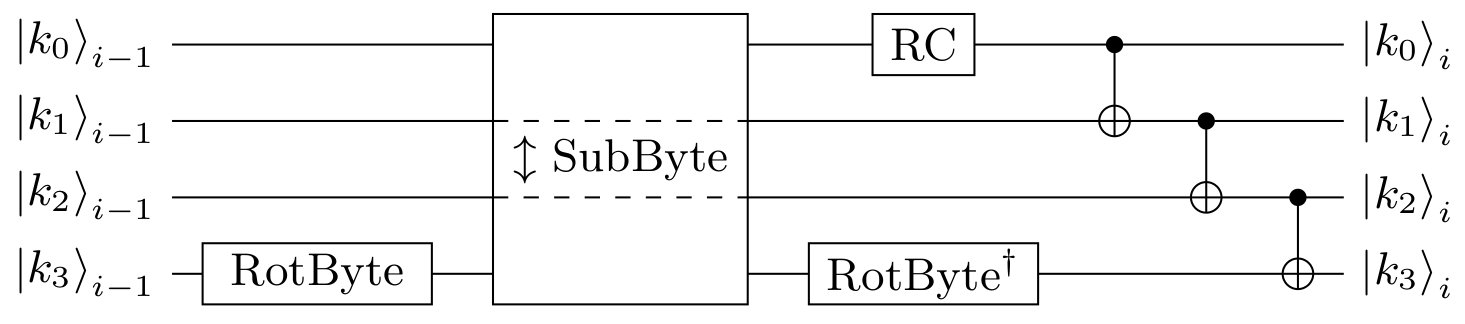
\includegraphics[width=\linewidth]{aes/aeske.png}
    \caption{AES-128 key expansion \cite{aeslowmc}}
    \label{fig:aeske}
\end{figure}
$\ket{k_j}_i$ represent the $j^{th}$ word (4 bytes) of the $i^{th}$ round key.
\end{frame}
\begin{frame}{QAES-128 circuit}
    \begin{figure}[h!]
    \centering
    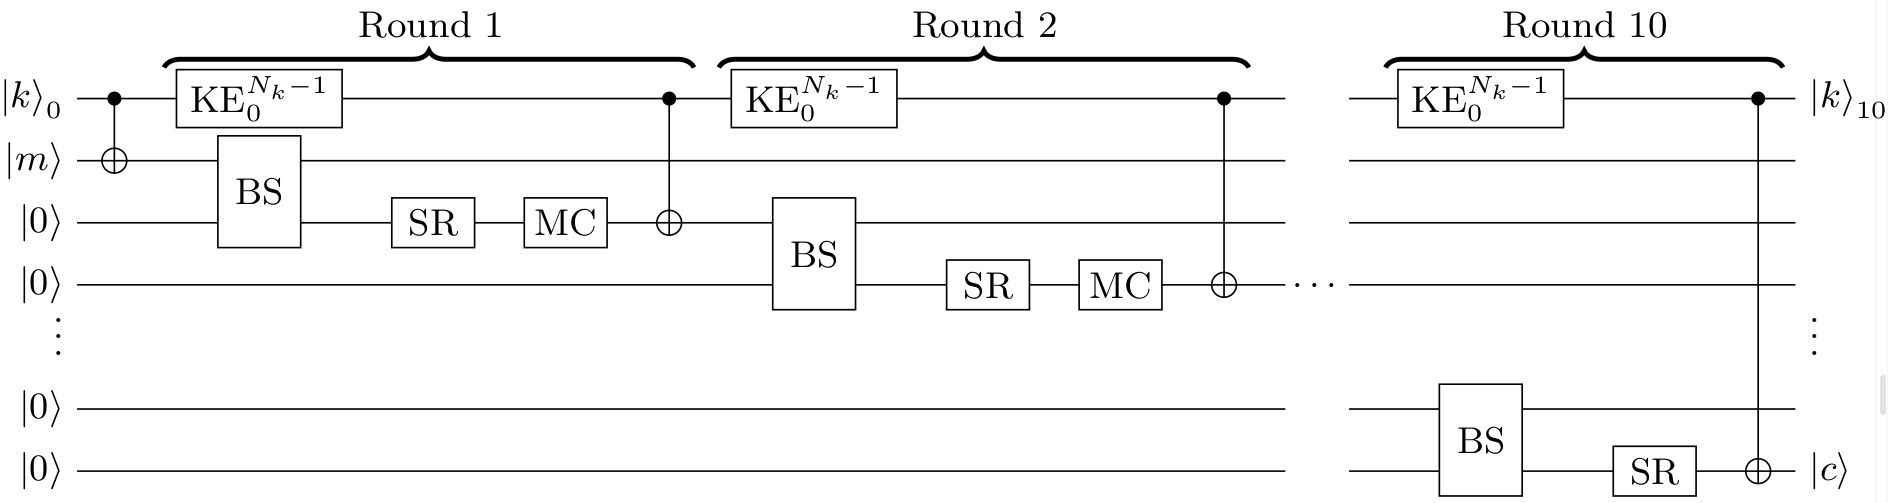
\includegraphics[width=\linewidth]{aes/aesfull.png}
    \caption{QAES-128 \cite{aeslowmc}}
    \label{fig:aesfull}
\end{figure}
Each wire represents 4 words (128 qubits). \pause $\ket{k}$ represents the master key and $\key{m}$ represents the message.\pause BS is Sbox, \pause SR is shift rows and \pause MC is mix column. Here we have used an in-place version of mix columns.
\begin{center}
\begin{table}[h!]
    \centering
    \resizebox{8cm}{!}{\begin{tabular}{ |c|c|c|c|c|c|c|c|c| } 
     \hline
     MC & CNOT & Clifford & T & M & T-depth & full depth & width & DW \\ \hline
    QAES-128 In place  & 2,91,150& 83,116&54,400&13,600&120&2,827&1,785&50,46,195 \\ \hline
     QAES-128 \cite{aesmc}\footfullcite{aesmc}  &2,93,730&83,236&54,400&13,600&120&2,094&2,937&61,50,078   \\ \hline
    \end{tabular}}
    \caption{QAES-128 cost of both variants of mix columns}
    \label{tab:aescost}
\end{table}
\end{center}
\end{frame}
\begin{frame}{Grover's Attack}
    \begin{figure}[h!]
    \centering
    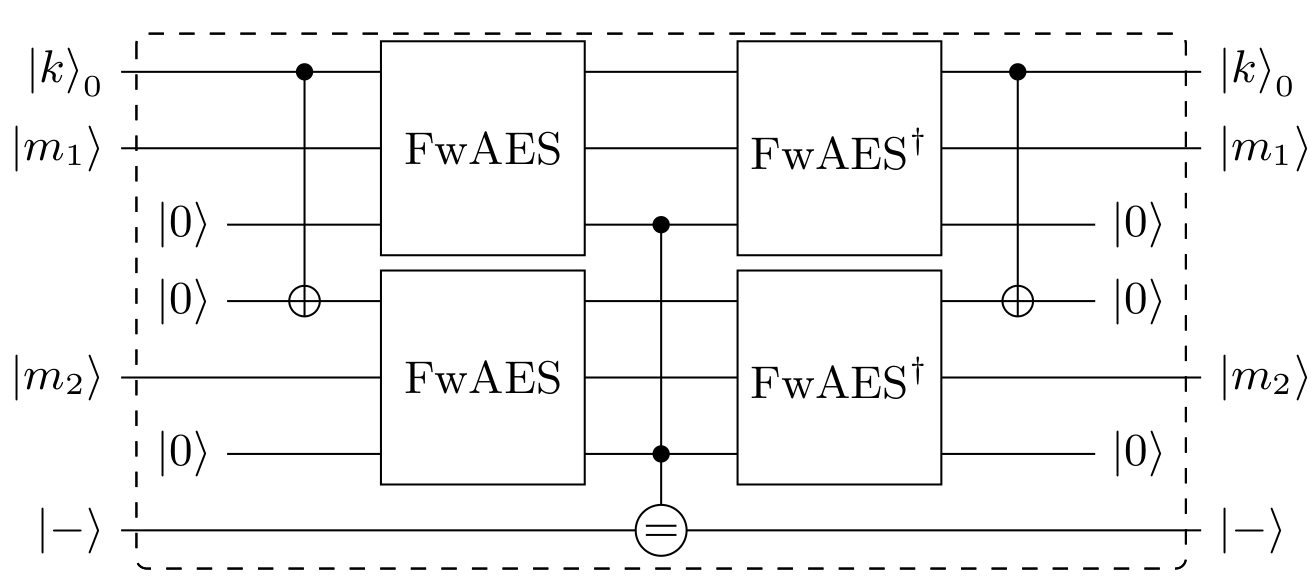
\includegraphics[width=\linewidth]{aes/aesrov.png}
    \caption{Grover's Attack on QAES-128 \cite{aeslowmc}}
    \label{fig:aesgrov}
\end{figure}
\begin{center}
\begin{table}[h!]
    \centering
    \resizebox{10cm}{!}{\begin{tabular}{ |c|c|c|c|c|c|c|c|c| } 
     \hline
     MC & CNOT & Clifford & T & M & T-depth & full depth & width & DW \\ \hline
    QAES-128 In place  & 5,85,051&1,69,184&1,09,820&27,455&121&2,815&3,329&93,71,135 \\ \hline
     QAES-128 \cite{aesmc}\footfullcite{aesmc}  & 5,89,643&1,68,288&1,09,820&27,455&121&2,096&5,633&1,18,06,768  \\ \hline
    \end{tabular}}
    \caption{QAES-128 Grover's Oracle cost of both variants of mix columns (r=2)}
    \label{tab:aesgrovcost}
\end{table}
\end{center}
\end{frame}
\begin{frame}{Cost Estimates}
    Let's calculate the cost estimates of Grover's Attack on QAES-128 in place with r = 2 with and without depth constraint.\pause
    \begin{equation*}
    \begin{aligned}
        G_G &= 5,85,051 + 1,69,184 + 1,09,820 + 27,455 = 8,91,510 \approx 1.7 \times 2^{19} \\ \pause
        G_D &= 2,815 \approx 1.37 \times 2^{11} \\ \pause
        G_W &= 3,329 \approx 1.62 \times 2^{11} \pause
    \end{aligned}
\end{equation*}\pause
Therefore the cost estimates without depth constraints keeping $S = 1$ is:\pause
\begin{equation*}
    \begin{aligned}
        D &\approx 1.37 \times 2^{11} \times 2^{64} = 1.37 \times 2^{75} \\ \pause
        G &\approx 1.7 \times 2^{19} \times 2^{64} = 1.7 \times 2^{83} \\\pause
        DW &\approx 1.37\times 2^{11} \times 1.62 \times 2^{11} \times 2^{64} \approx 1.1 \times 2^{87}
    \end{aligned}
\end{equation*}
\pause
Similarly, the cost estimates with depth constraint of $2^{40}$ are: \pause
\begin{equation*}
    \begin{aligned}
        S &\approx 2^{128}\times 1.37^2 \times 2^{22} \times 2^{-80} \approx 1.87 \times 2^{70} \\ \pause
        G &\approx 2^{128} \times 1.37 \times 2^{11} \times 1.7 \times 2^{19} \times 2^{-40} \approx 1.16 \times 2^{119} \\ \pause
        DW &\approx 2^{128} \times 1.37^2 \times 2^{22} \times 1.62 \times 2^{11} \times 2^{-40} \approx 1.52 \times 2^{122} 
    \end{aligned} 
\end{equation*}
\end{frame}
\begin{frame}{Cost Estimates Contd.}
    \begin{itemize}
        \item NIST\cite{nist}\footfullcite{nist}  has proposed a maximum of $2^{170}/$MAXDEPTH quantum gates for AES-128 but this does not take into account the effects of parallelization. \pause
        \item For MAXDEPTH = $2^{40}$, \cite{nist} has bounded the count of quantum gates by $2^{170}/2^{40} = 2^{130}$. \pause
        \item From the above calculation of G-cost we can see that the number of gates required by AES-128 is much less after parallelization ($2^{119}$). 
    \end{itemize}
\end{frame}